\documentclass[conference]{IEEEtran}
\IEEEoverridecommandlockouts
% The preceding line is only needed to identify funding in the first footnote. If that is unneeded, please comment it out.
\usepackage{cite}
\usepackage{amsmath,amssymb,amsfonts}
\usepackage{algorithmic}
\usepackage{graphicx}
\usepackage{textcomp}
\usepackage{xcolor}
\usepackage{listings}

\def\BibTeX{{\rm B\kern-.05em{\sc i\kern-.025em b}\kern-.08em
    T\kern-.1667em\lower.7ex\hbox{E}\kern-.125emX}}
\begin{document}

\title{CENG435 Term Project-1 Report\\
{\footnotesize}
}

\author{\IEEEauthorblockN{Name Surname : Omer CETIN}
\IEEEauthorblockA{Student ID : 2257541 \\
}
\and
\IEEEauthorblockN{Name Surname : Oguzcan BUDUMLU}
\IEEEauthorblockA{Student ID : 2098820
}
}

\maketitle
\section{Introduction}\\
In this homework, we implemented our Reliable Data Transfer (RDT) protocol on top of transport layer protocol UDP. The implemented protocol also supports pipelining and multihoming. In order to use routers as gateways in file transfer paths from source to destination, we configured them  with commands explained in Routing Mechanism section. \\
\\
We used Python programming language for implementation because of its convenience in socket programming and we used its some libraries: \textit{threading} for multi-homing functionality, \textit{hashlib} for checksum, \textit{time} for timeouts, \textit{datetime} for querying local time.\\
\\
For experiments and testing our protocol, we used a sample file whose size is 5 megabytes. We compared checksum of sample file in source and  checksum of obtained file in destination using $md5sum$ command in Linux. After each transmission, we compared file in source with created file in destination. During all our experiments, we did not encountered a wrong situtation.\\
\\
\textbf{\textit{We did all parts of homework together.}}
\section{Understanding The Topology}\\
\begin{figure}[ht]
  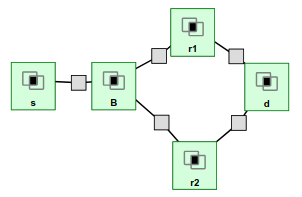
\includegraphics[width=\linewidth]{topology.png}
  \caption{Topology}
  \label{fig:boat1}
\end{figure}
In our topology, there are five nodes which have different roles in our network that we have built.\\
s node is the source that is simply the source of data and where the data is being sent over TCP to the broker.\\
B node is the broker which collects packets which will create file from source via TCP and creates a temporary file to send it to d node via our reliable data transfer protocol which is on top of UDP.\\
r1 and r2 are routers and so gateways for file transfer. We configured them in the way mentioned in Routing Mechanism Section.\\
d is the destination which receives packets of file and send acknowledgment packets for received packets to broker node via routers.\\
\section{Overview of Protocol}\\
After transferring file from source to broker, we send half of the file from broker to destination via r1, and we send other half of the file from broker to destination via r2. In response to this, for data packets received via r1, acknowledgment packets is sent via r1 from the destination. Similary, for data packets received via r2, acknowledgment packets is sent via r2 from the destination. In a nutshell, while one path deals with half of the file, another path deals with other part of file.Therefore, we create two threads in the broker and destination.We provide \textbf{multihoming} in such a way.\\
\\
We used go-back-n strategy in our protocol for \textbf{pipelining}.\\
It would be better to be explained by point of views of broker and destination separately for a better understanding of the protocol.\\
From the point of view of the broker:\\
Firstly we send a packet with a sequence number and checksum (say them header information) and we store it in a window list (in window we hold packets that is sent but not ACKed). We
 wait an ACK for sent packet.If after some time (as timeout) ACK does not come, we send one more packet with its header information. If we assume that we never receive ACK, we send packets up to number of window size.\\
That brings us to point of \textbf{pipelining}.\\
\\
After sending packets as number of window size, if we do not receive an ACK packet, because of the probability of packet loss,  we send all packets in window again (\textbf{retransmission}).\\
\\
 If we receive an ACK with ackNumber n, we say that packets which have sequence number up to n are transmitted successfully(cumulative acknowledgement concept). After that, we remove sent packets from window list and we increase window base number, which limits maximum number of sent but not ACKed packets, up to  n.
\\
In each iteration of sending packets, we compare sequence number with number of packet that needs to be sent in total. If they are equal and also there is no packet in window, we can say that all packets are sent and there is no remaining packet that needs to be ACKed. Hence, we terminate packet transmit stage and we send FIN packets until it is ACKed from the destination.\\
\\
\\
We should mention some missing points through the eyes of destination:\\
Destination sends ACK packets but condition of this action is that expected sequence number should be equal to sequence number of coming packet. If not, we discard coming packet. If we assume there is no coming packet, timeout occurs and we send an ACK with expected sequence number.We should remind that expected sequence number tells us all packets came up to this number (not including this number).\\We should emphasize that this ACK mechanism is all about \textbf{reliability}.\\
\\
Finishing action is determined by the sender. Like mentioned above, if necessary conditions hold, the broker sends FIN packet. After destination receives this packet, it sends one more packet with expected sequence number.This implies it received FIN packet and it finishes receiving operation and combines two collection (because of two threads) in  file with name "output.txt".\\
\\
Duration of all process explained, we used md5 for \textbf{checksum} of each packet transmitted from broker to destination or vice versa.\\
\\
We should also note that all mechanism and methodology explained above is valid for each thread. We divided file into two parts equally in size and assigned each thread for each part to send it successfully to destination. This provides \textbf{multihoming} as explained above also.\\
\\

After explaining overall implementation of our protocol, we should collect important points as a summary:\\
\begin{itemize}
\item For reliable data transfer, we used checksum, retransmission, sequence number, cumulative ACK mechanism and windowing.
\item In order to handle packet loss, we used cumulative ACK concept and timeout. Unless expected data packet is not received by the destination, this unexpected packet is discarded and ACK packet with expected sequence number is sent by the destination. If a packet is not ACKed for a while, the broker is timed-out and resends packets in window. When the destination does not receive a packet for a while, it is also timed-out and send a ACK packet with expected sequence number.
\item In order to handle corruption, we used checksum. Each transferred packet in both direction is processed with checksum operation.
\item In order to handle reordering issue, we used sequence number. At destination side, the packet which comes out of sequence is discarded.
\end{itemize}





\section{Routing Mechanism}
We configured routers such that data packets which comes from broker host are transferred to destination host and acknowledgment packets which comes from destination host are transferred to broker host. In other words, routers are gateways. They look destination IP of packets and determine which interface packets need to be transferred.\\
For this purpose, we used $route$ command.The general form of command with an example:\\
\begin{lstlisting}[language=bash]
  $ route add -host <targetInterfaceIP>
  dev <usedInterface>
  $ route add -host 10.10.2.1 dev eth1
\end{lstlisting}
Here, router transfers the incoming packet whose destination IP is $10.10.2.1$ via eth1 interface.\\
Also in order to make use of gateway, $route$ command is used in the following manner:
\begin{lstlisting}[language=bash]
  $ route add -host <targetInterfaceIP> 
  gw <gatewayInterfaceIP> dev <usedInterface>
\end{lstlisting}\\
This command is used in the broker to adjust routers as gateways.\\
\\
r1 and r2 are adjusted as gateways seperately.We used following commands in the broker:
\begin{lstlisting}[language=bash]
  $ route add -host 10.10.5.2 gw 
  10.10.4.2 dev eth3
  $ route add -host 10.10.3.2 gw 
  10.10.2.2 dev eth2
\end{lstlisting}\\
We used following commands in r1.
\begin{lstlisting}[language=bash]
  $ route add -host 10.10.2.1 dev eth1
  $ route add -host 10.10.3.1 dev eth2
\end{lstlisting}\\
We used following commands in r2.
\begin{lstlisting}[language=bash]
  $ route add -host 10.10.4.1 dev eth1
  $ route add -host 10.10.5.2 dev eth2
\end{lstlisting}
\\
After this set up process, routing tables in nodes are:\\
\begin{figure}[ht]
  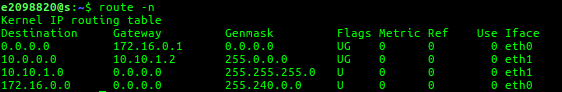
\includegraphics[width=\linewidth]{s.png}
  \caption{Source node}
  \label{fig:boat1}
    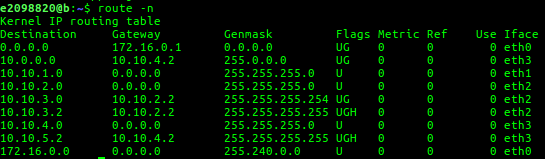
\includegraphics[width=\linewidth]{b.png}
  \caption{Broker node}
  \label{fig:boat1}
    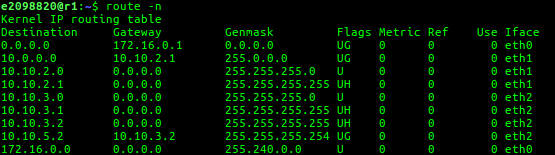
\includegraphics[width=\linewidth]{r1.png}
  \caption{r1 node}
  \label{fig:boat1}
    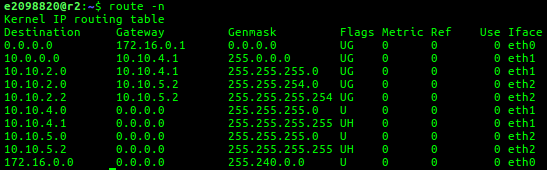
\includegraphics[width=\linewidth]{r2.png}
  \caption{r2 node}
  \label{fig:boat1}
\end{figure}
\begin{figure}[ht]
  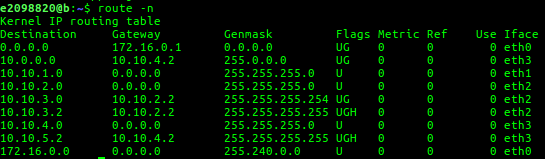
\includegraphics[width=\linewidth]{b.png}
  \caption{Broker node}
  \label{fig:boat1}
    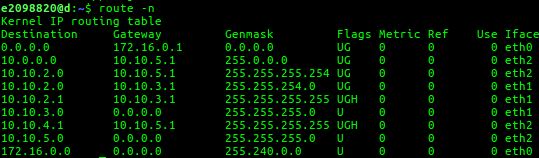
\includegraphics[width=\linewidth]{d.png}
  \caption{Destination node}
  \label{fig:boat1}
\end{figure}
\\
\\
\\
\\

\section{Experiment}
There are 3 experiments we have to do. In each experiment, we add a specific delay to the broker and routers with executing netem/tc commands on virtual machines. In the first experiment we add 1ms delay, in the second 20 milliseconds and in the third 60 milliseconds with 5 milliseconds normal distribution.
We have plotted the below graph according to results of the each experiment performed. \\
\begin{figure}[ht]
  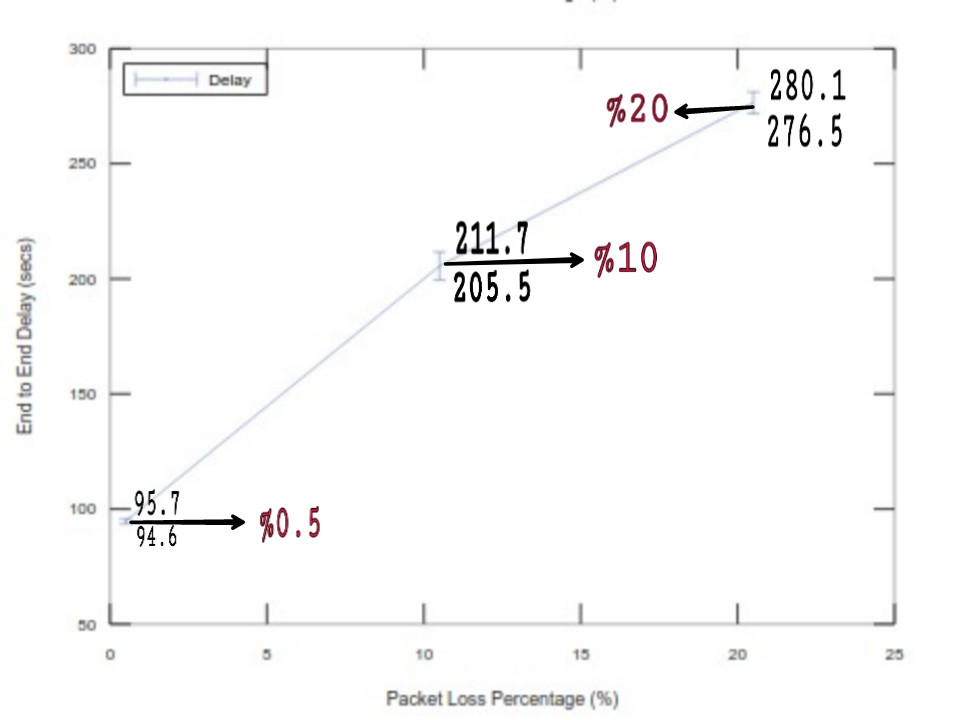
\includegraphics[width=\linewidth]{loss.jpeg}
  \caption{Packet Loss}
  \label{fig:boat1}
\end{figure}\\

The graph above shows the relationship between end to end delay and packet loss percentage. As seen in the graph, when we increased the percentage of the packet loss, the end to end delay increases, because the packets should be sent again until they are acknowledged. In the first part of this experiment, we arranged the packet loss percentage as \%0.5 and the end to end delay was around (95.1+-0.5). In the second part of the experiment, we arranged the packet loss percentage as \%10 and the end to end delay was around (208.6+-3.1). In the third part of the experiment, we arranged the packet loss percentage as \%20 and the end to end delay was around (278,3+-1.8). Lastly, when we have the packet lost along the way to the destination, the tranferring process took much longer time. 

\begin{figure}[ht]
  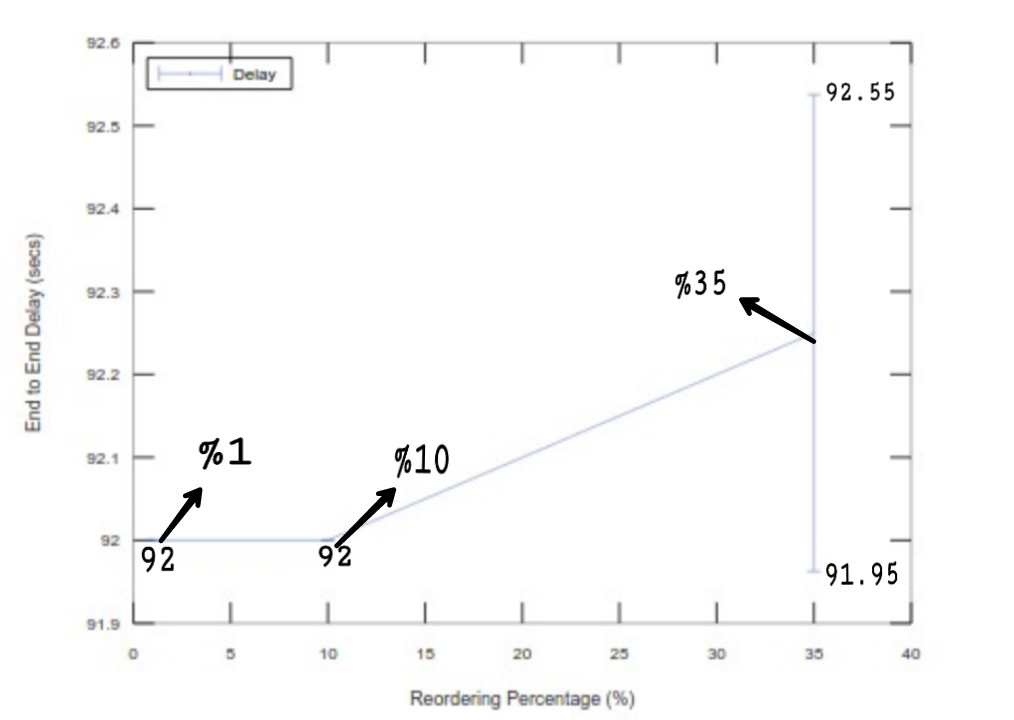
\includegraphics[width=\linewidth]{reordering.jpeg}
  \caption{Packet Reordering}
  \label{fig:boat1}
\end{figure}\\

The graph above shows the relationship between end to end delay and packet reordering percentage. As seen in the graph, when we increased the percentage of the packet reordering, the end to end delay increases. In the first part of this experiment, we arranged the packet reordering percentage as \%1 and the end to end delay was 92. In the second part of the experiment, we arranged the packet loss percentage as \%10 and the end to end delay was 92. In the third part of the experiment, we arranged the packet loss percentage as \%35 and the end to end delay was around (92.25+-0.3). Lastly, we see that our protocol can tolerate the packet reordering quite well.

\begin{figure}[ht]
  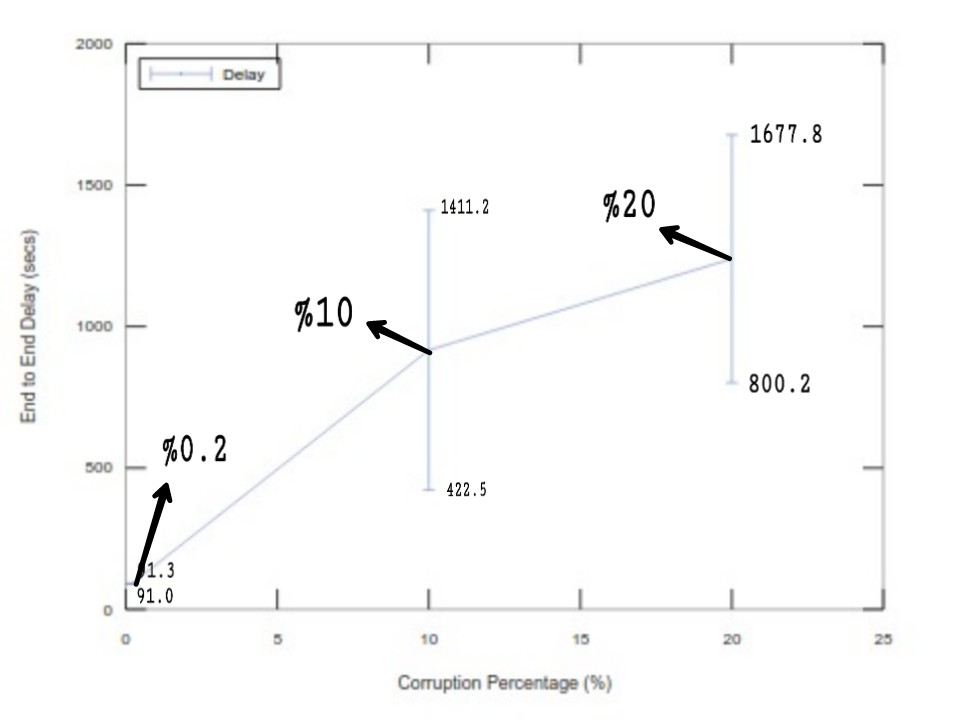
\includegraphics[width=\linewidth]{corruption.jpeg}
  \caption{Packet Corruption}
  \label{fig:boat1}
\end{figure}\\

The graph above shows the relationship between end to end delay and packet corruption percentage. As seen in the graph, when we increased the percentage of the packet corruption, the end to end delay increases because the packets should be sent again until they are acknowledged. In the first part of this experiment, we arranged the packet corruption percentage as \%0.2 and the end to end delay was (91.0+-0.15). In the second part of the experiment, we arranged the packet corruption percentage as \%10 and the end to end delay was (916.8+-494.3). In the third part of the experiment, we arranged the packet corruption percentage as \%20 and the end to end delay was around (1239+-438.8). Lastly, we see that when we increase the packet corruption percentage from \%0.2 to \%10 like 50 times, the end to end delay error interval increases dramatically. Plus when we increase the packet corruption, the end to end delay increased as expected.

\end{document}
